%%%%%%%%%%%%%%%%%%%%%%%%%%%%%%%%%%%%%%%%%%%%%%%%%%%%%%%%%%%%%%%%%%%%%
%
% CSCI 1430 Writeup Template
%
% This is a LaTeX document. LaTeX is a markup language for producing
% documents. Your task is to fill out this
% document, then to compile this into a PDF document.
%
% TO COMPILE:
% > pdflatex thisfile.tex
%
% For references to appear correctly instead of as '??', you must run
% pdflatex twice.
%
% If you do not have LaTeX and need a LaTeX distribution:
% - Departmental machines have one installed.
% - Personal laptops (all common OS): www.latex-project.org/get/
%
% If you need help with LaTeX, please come to office hours.
% Or, there is plenty of help online:
% https://en.wikibooks.org/wiki/LaTeX
%
% Good luck!
% James and the 1430 staff
%
%%%%%%%%%%%%%%%%%%%%%%%%%%%%%%%%%%%%%%%%%%%%%%%%%%%%%%%%%%%%%%%%%%%%%
%
% How to include two graphics on the same line:
%
% \includegraphics[\width=0.49\linewidth]{yourgraphic1.png}
% \includegraphics[\width=0.49\linewidth]{yourgraphic2.png}
%
% How to include equations:
%
% \begin{equation}
% y = mx+c
% \end{equation}
%
%%%%%%%%%%%%%%%%%%%%%%%%%%%%%%%%%%%%%%%%%%%%%%%%%%%%%%%%%%%%%%%%%%%%%%%%%%%%%%%%%%%%%%%%%%%%%%%%

\documentclass[11pt]{article}

\usepackage[english]{babel}
\usepackage[utf8]{inputenc}
\usepackage[colorlinks = true,
            linkcolor = blue,
            urlcolor  = blue]{hyperref}
\usepackage[a4paper,margin=1.5in]{geometry}
\usepackage{stackengine,graphicx}
\usepackage{fancyhdr}
\setlength{\headheight}{15pt}
\usepackage{microtype}
\usepackage{times}
\usepackage{booktabs}

% python code format: https://github.com/olivierverdier/python-latex-highlighting
\usepackage{pythonhighlight}

\frenchspacing
\setlength{\parindent}{0cm} % Default is 15pt.
\setlength{\parskip}{0.3cm plus1mm minus1mm}

\pagestyle{fancy}
\fancyhf{}
\lhead{Homework 5 Writeup}
\rhead{CSCI 1430}
\rfoot{\thepage}

\date{}

\title{\vspace{-1cm}Homework 5 Writeup}


\begin{document}
\maketitle
\vspace{-2cm}
\thispagestyle{fancy}

\section*{Instructions}
\begin{itemize}
  \item Provide an overview about how your project functions. 
  \item Describe any interesting decisions you made to write your algorithm.
  \item Show and discuss the results of your algorithm.
  \item Feel free to include code snippets, images, and equations.
  \item List any extra credit implementation and result (optional).
  \item Use as many pages as you need, but err on the short side.
  \item \textbf{Please make this document anonymous.}
\end{itemize}

\section*{Project Overview}

This project is about training a convolutional neural network to perform scene
classification. We train a head on a pre-trained model, and create and train a
model from scratch.

\section*{Implementation Detail}

\section*{Result}

\begin{figure}[h]
    \centering
    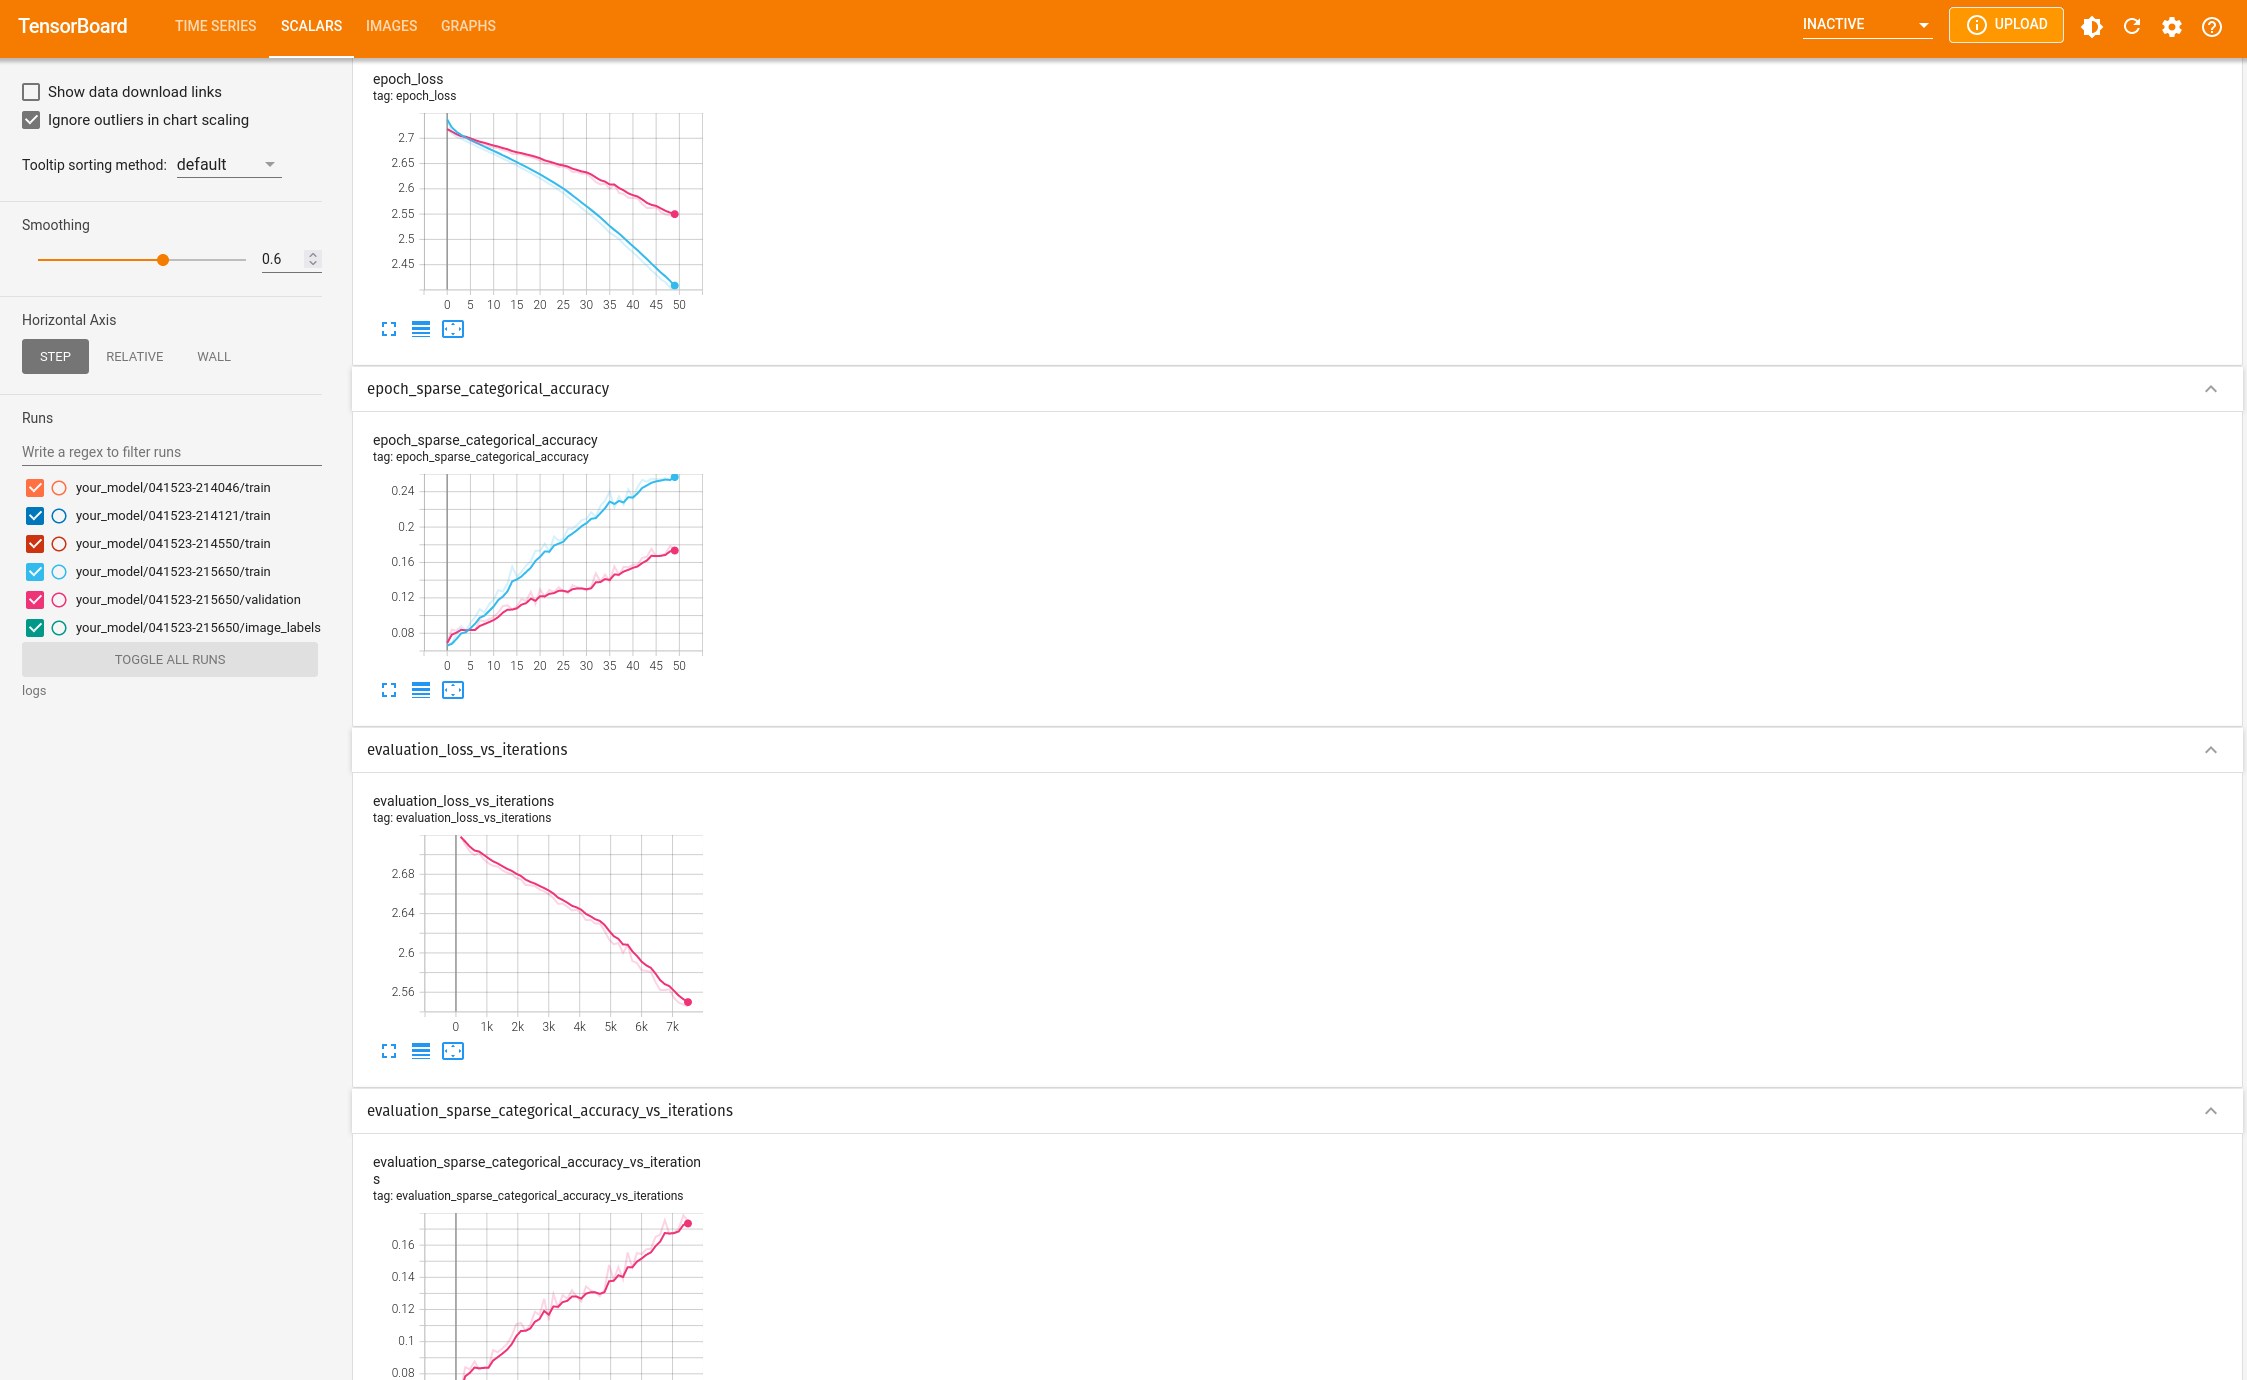
\includegraphics[width=5cm]{task1v0-2.png}
    \caption{Task 1:Training the small model on CPU. Somehow this was very fast.}
    \label{fig:result1}
\end{figure}


\begin{figure}[h]
    \centering
    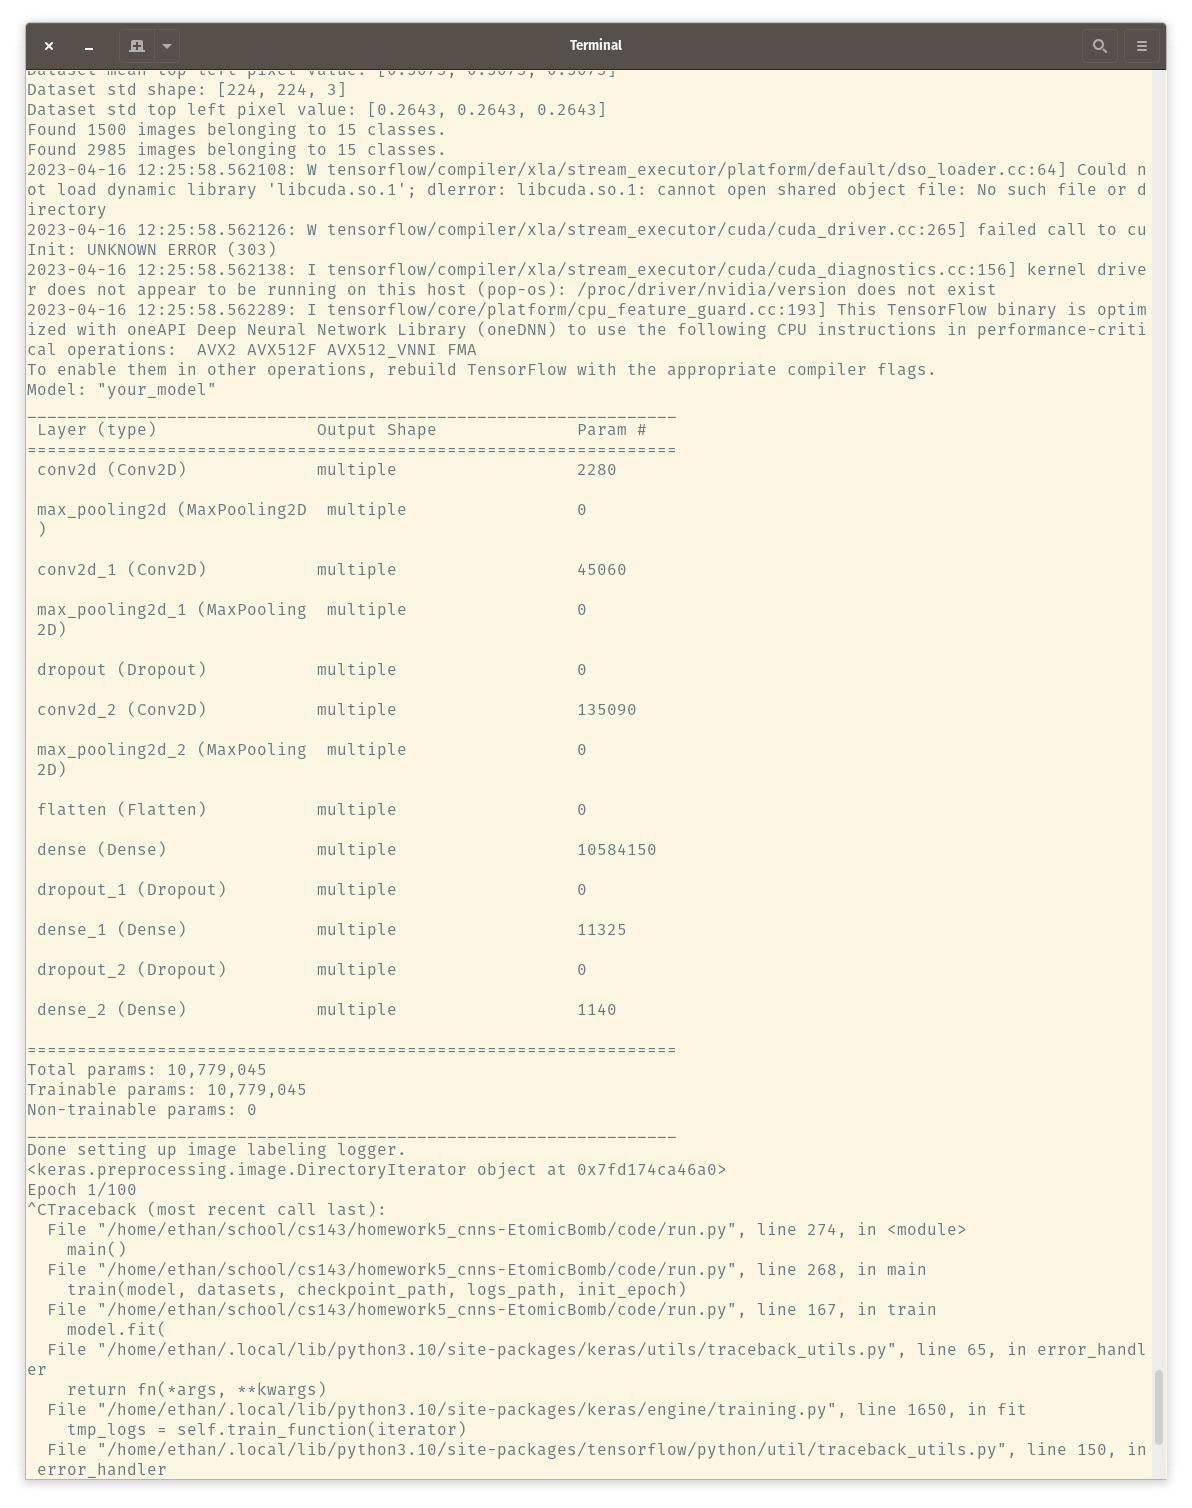
\includegraphics[width=5cm]{complete-parameters.png}
    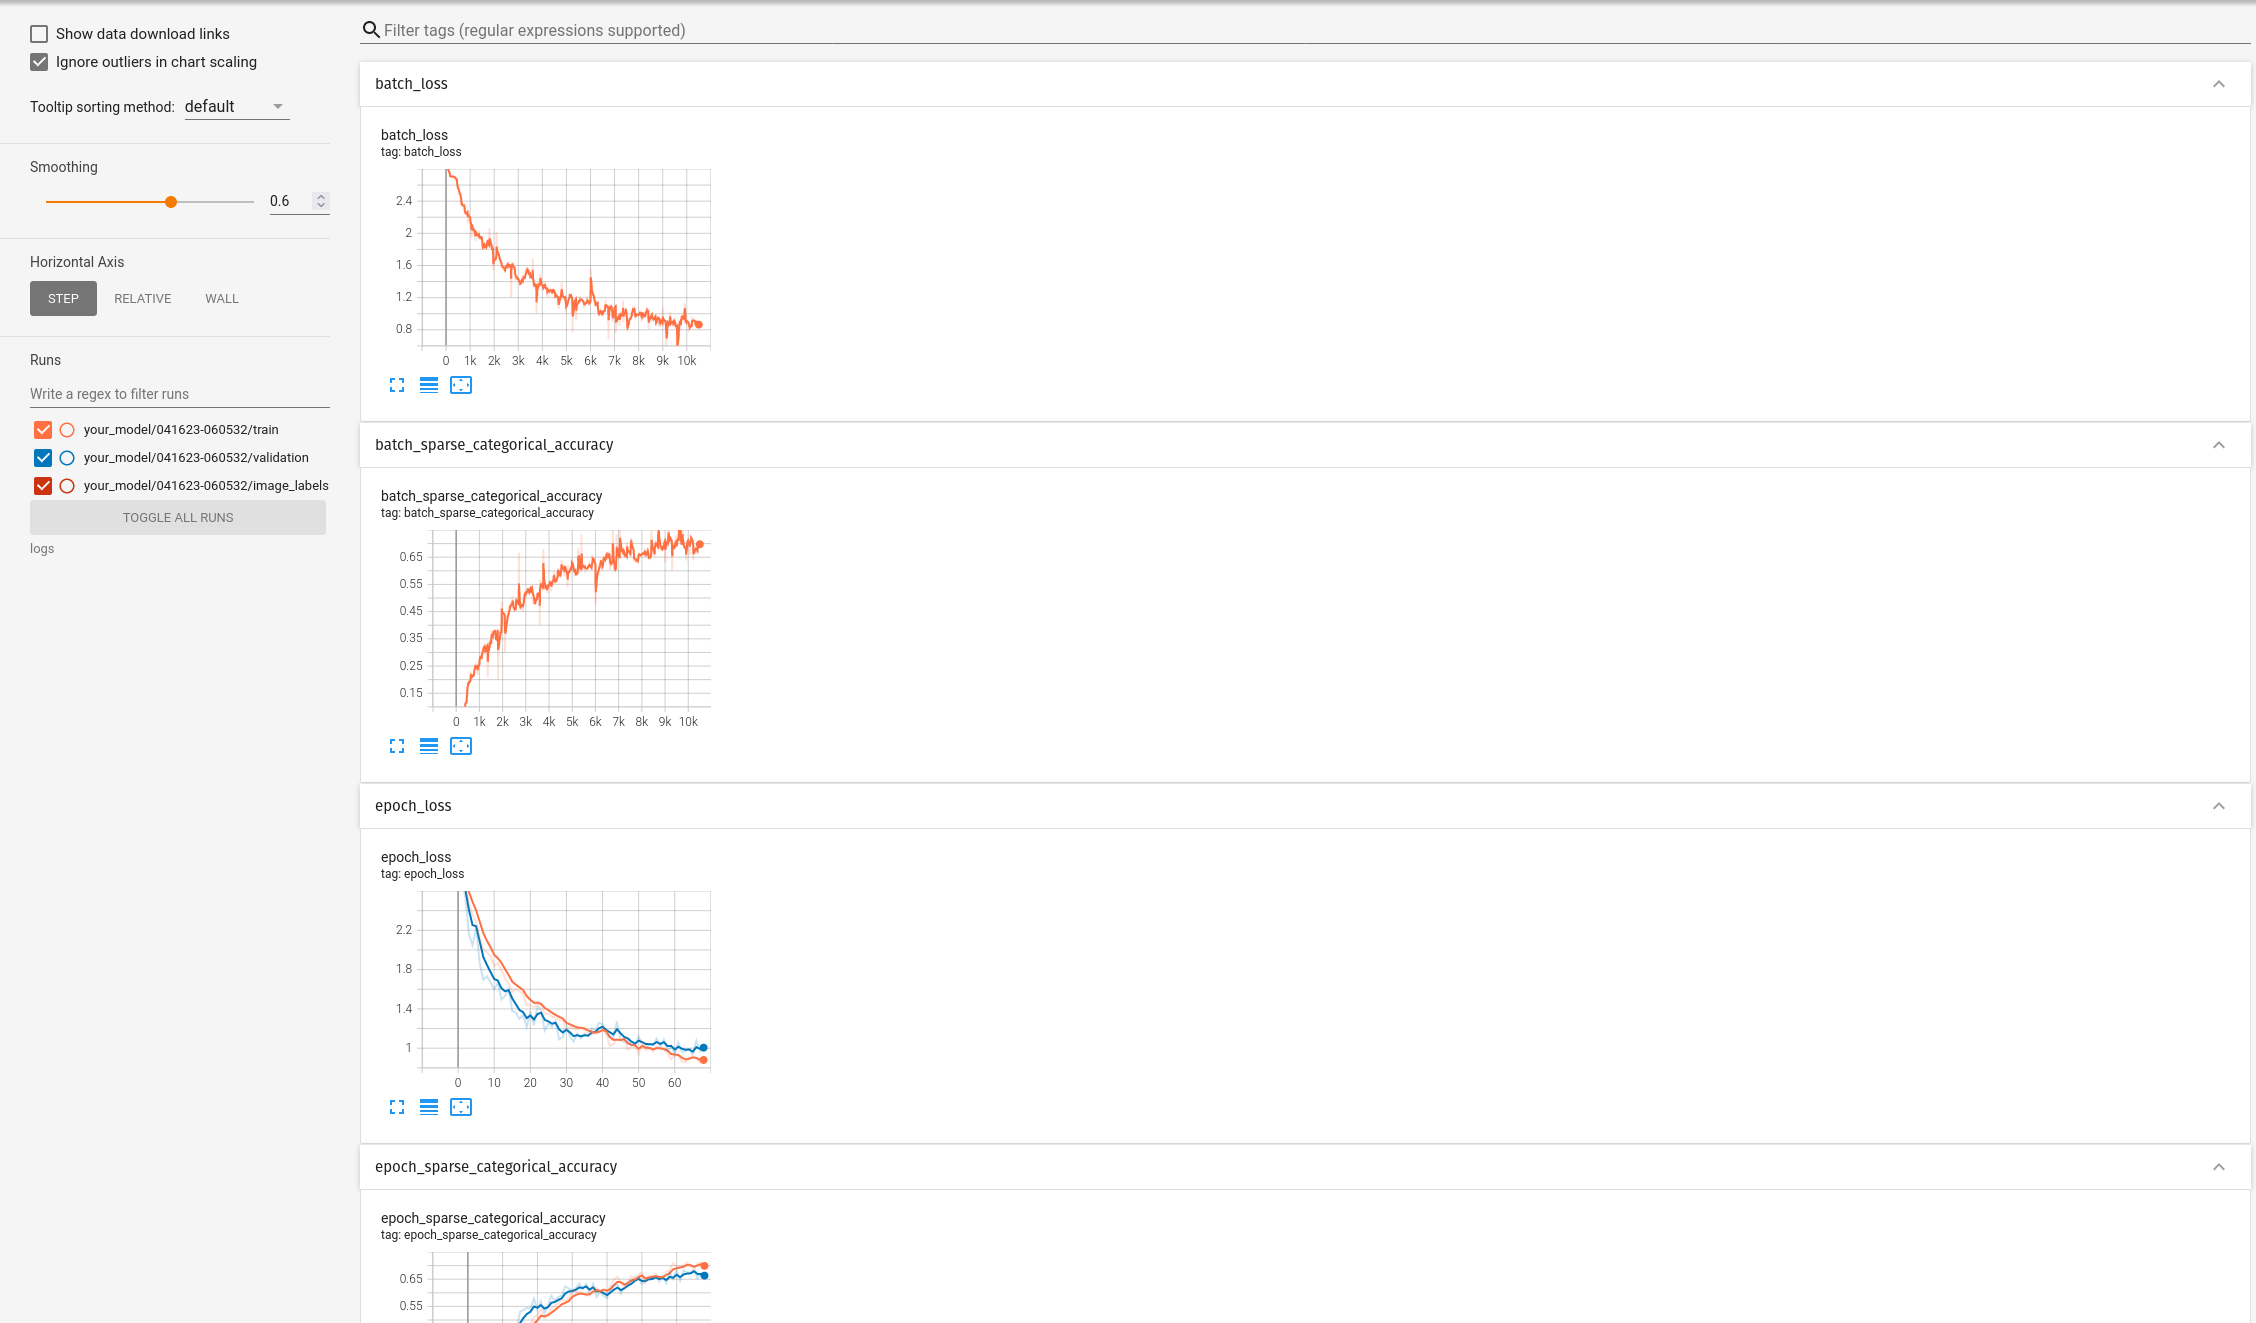
\includegraphics[width=5cm]{complete-a.png}
    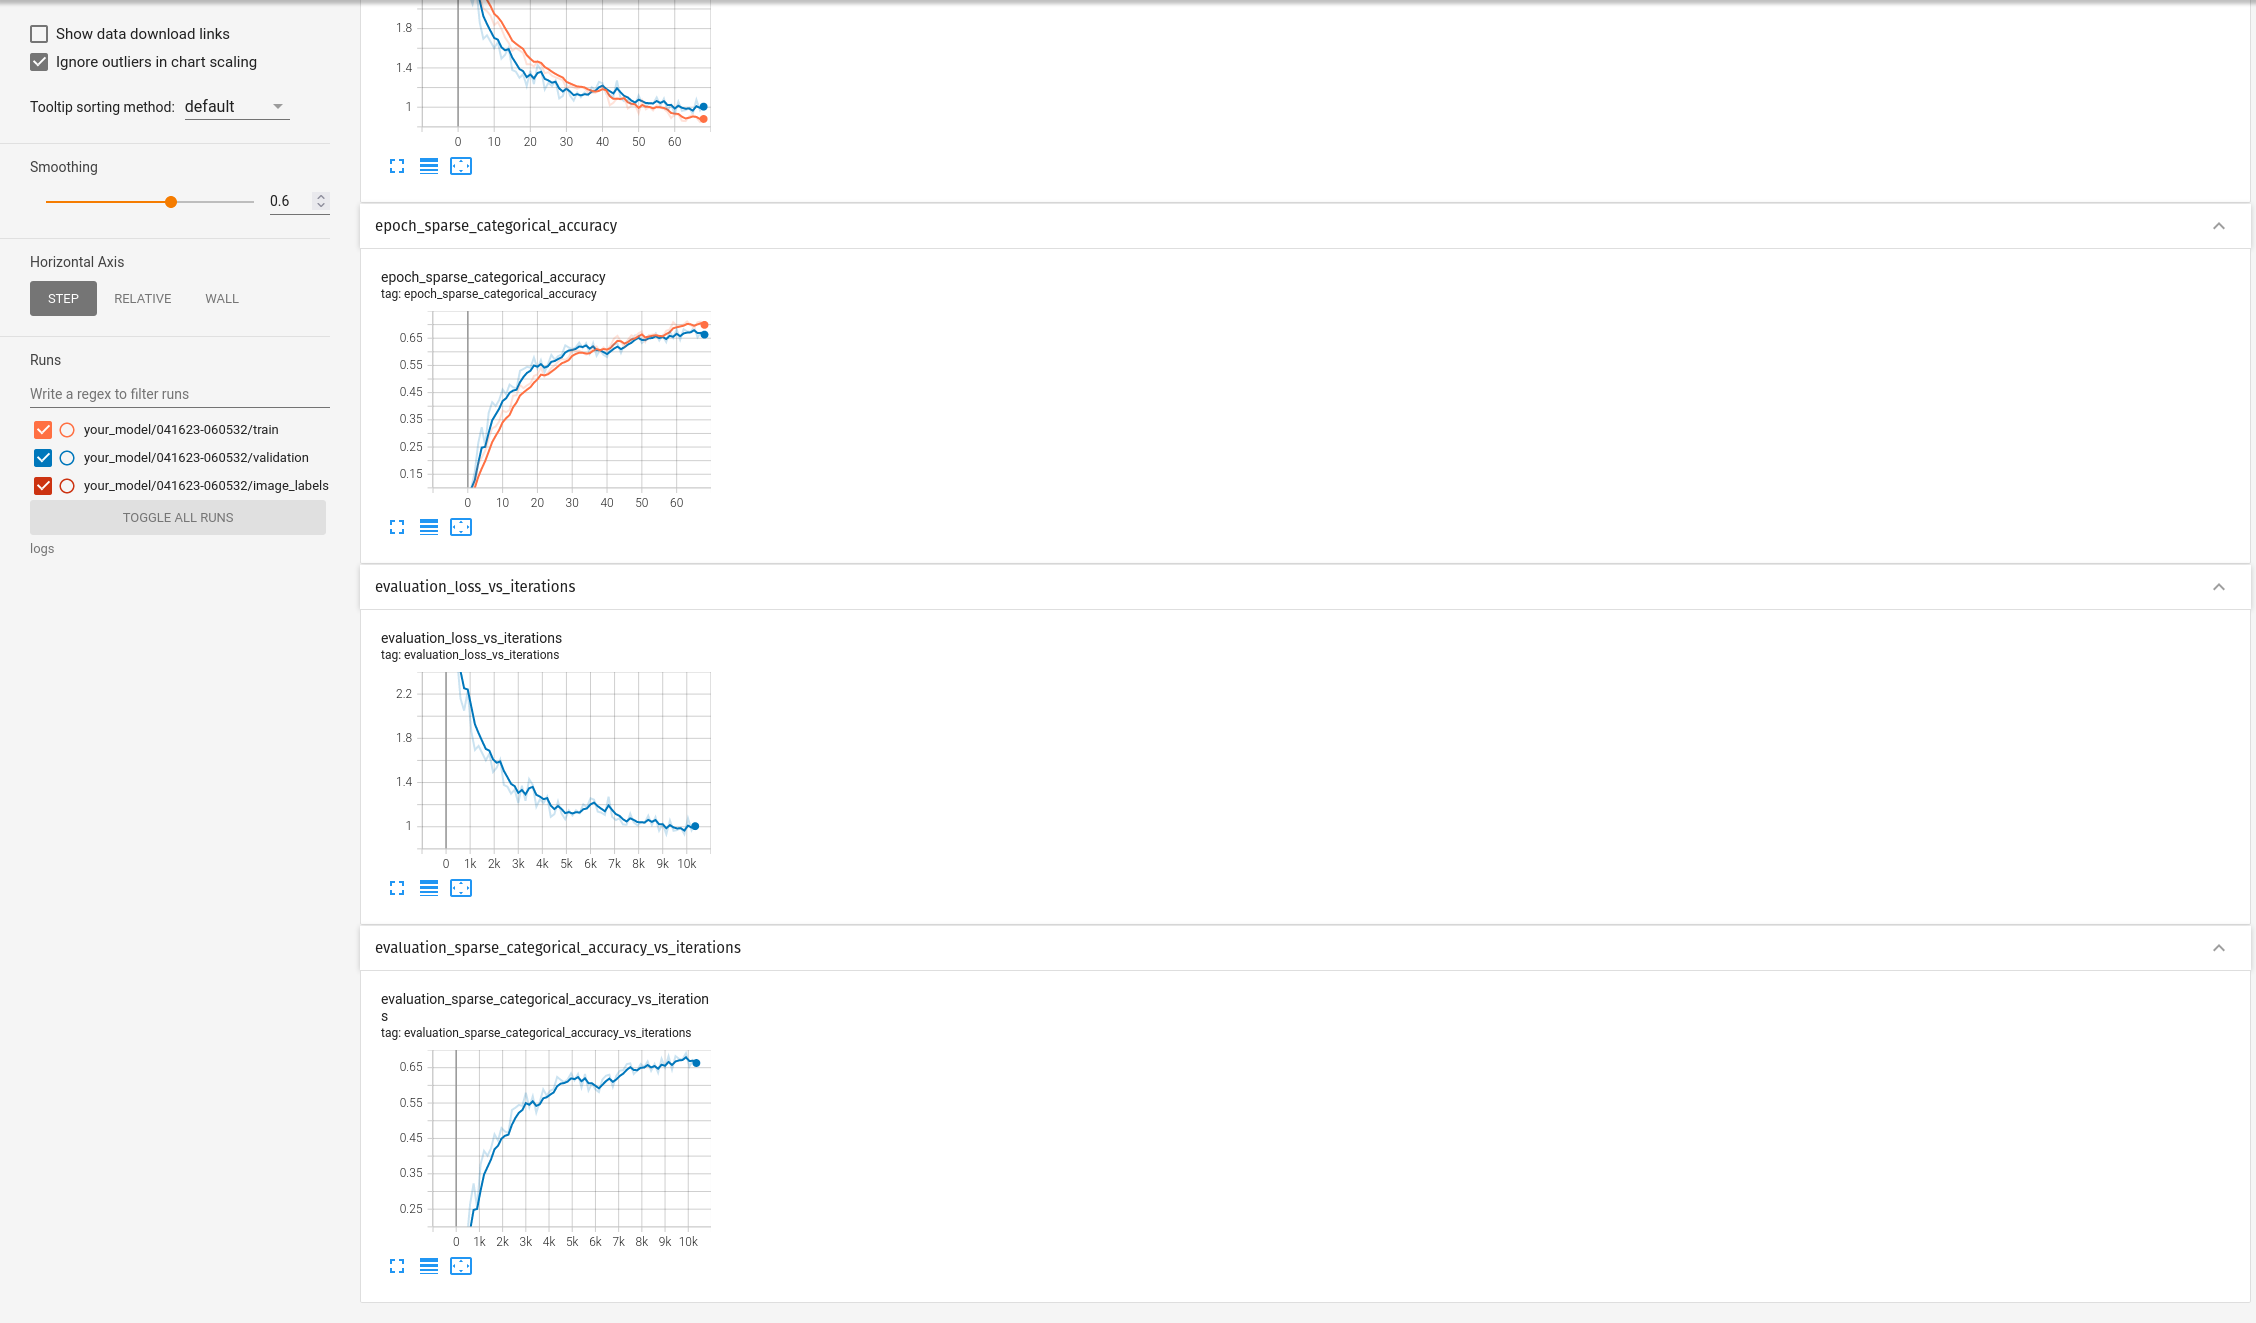
\includegraphics[width=5cm]{complete-b.png}
    \caption{Progress training the complete model}
    \label{fig:result1}
\end{figure}

\begin{figure}[h]
    \centering
    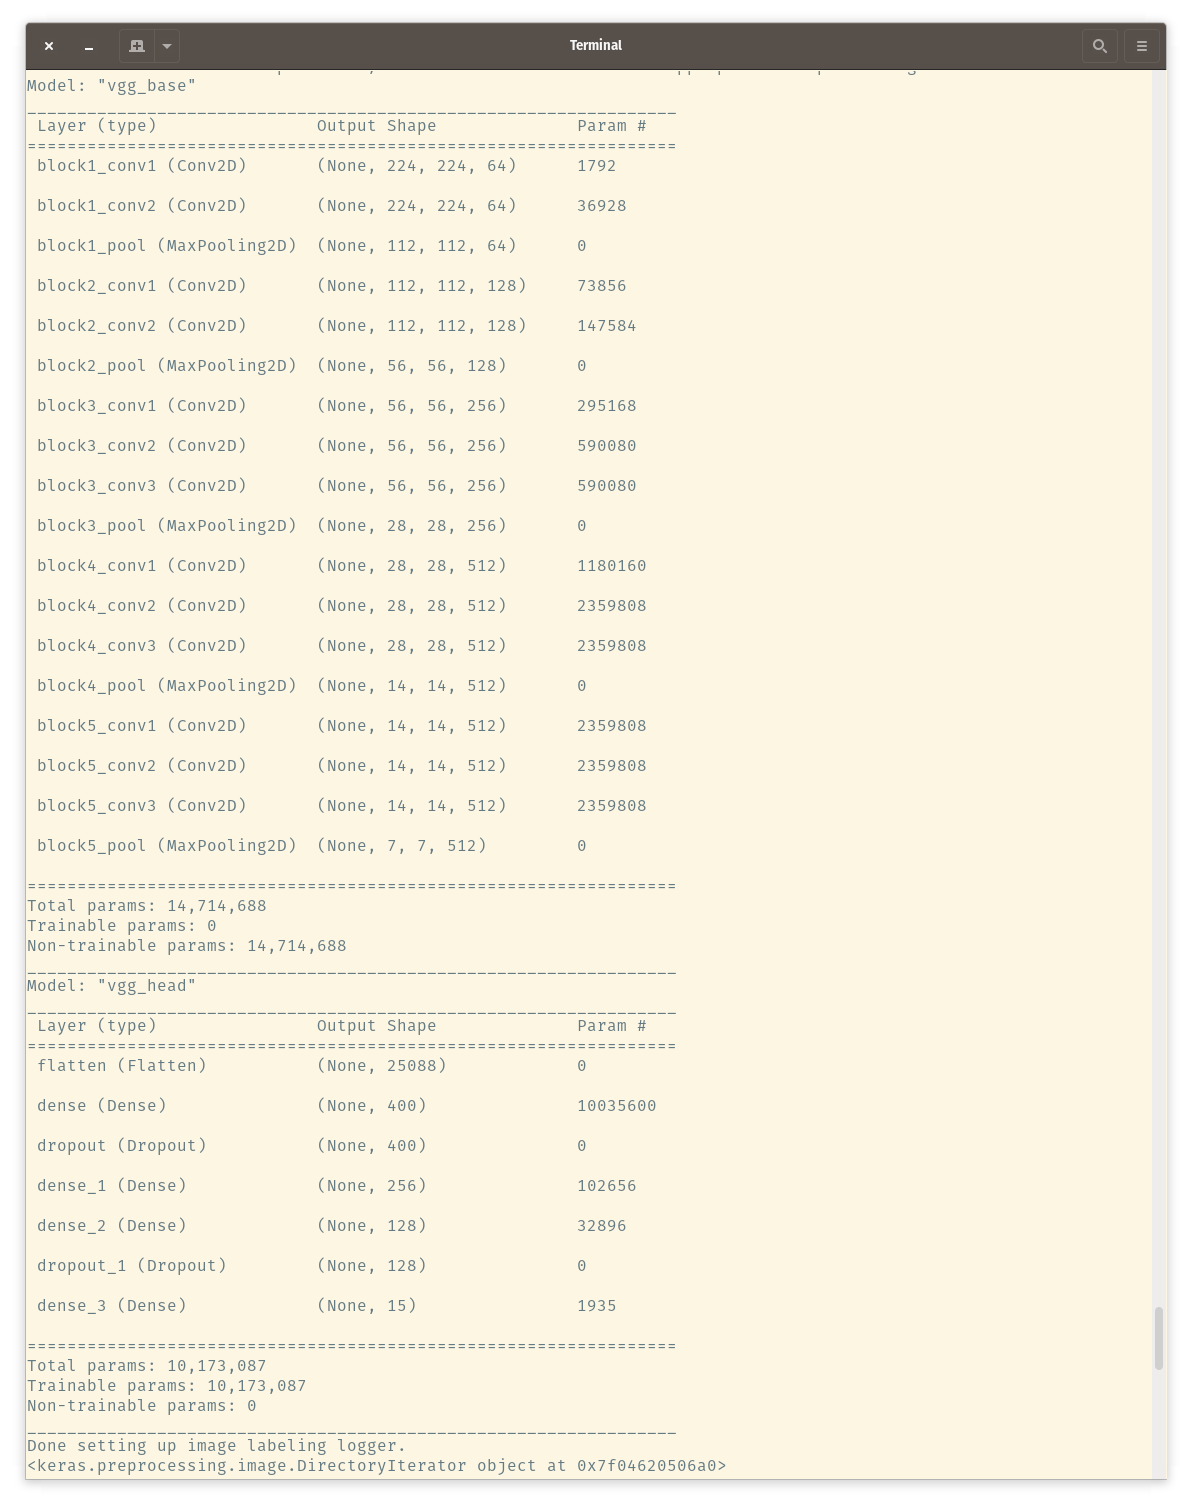
\includegraphics[width=5cm]{vgg-parameters.png}
    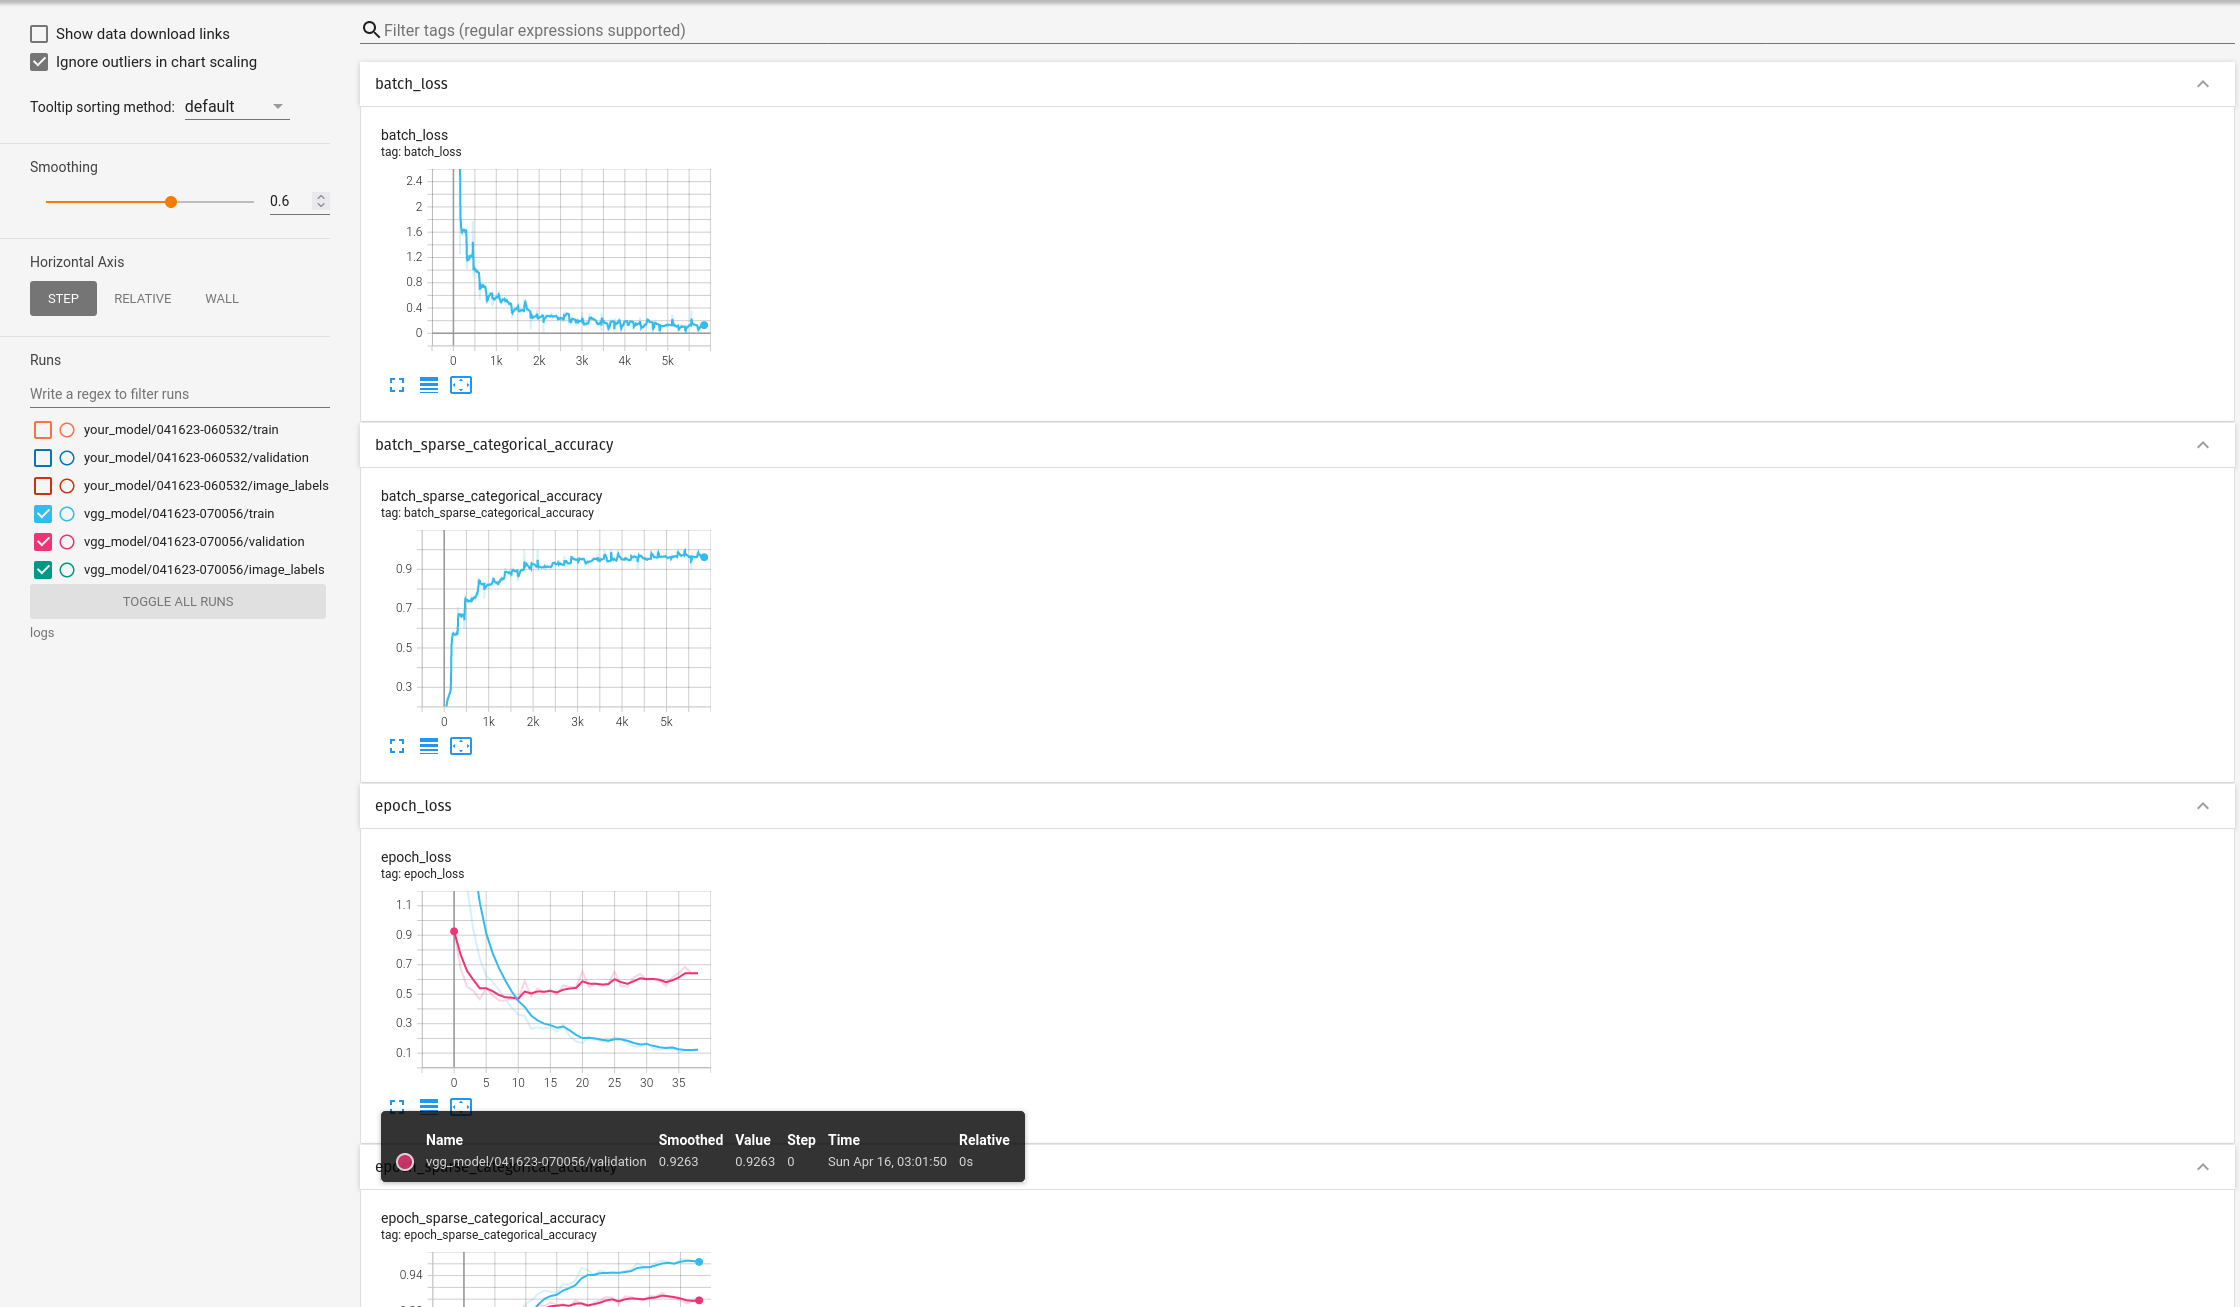
\includegraphics[width=5cm]{vgg-a.png}
    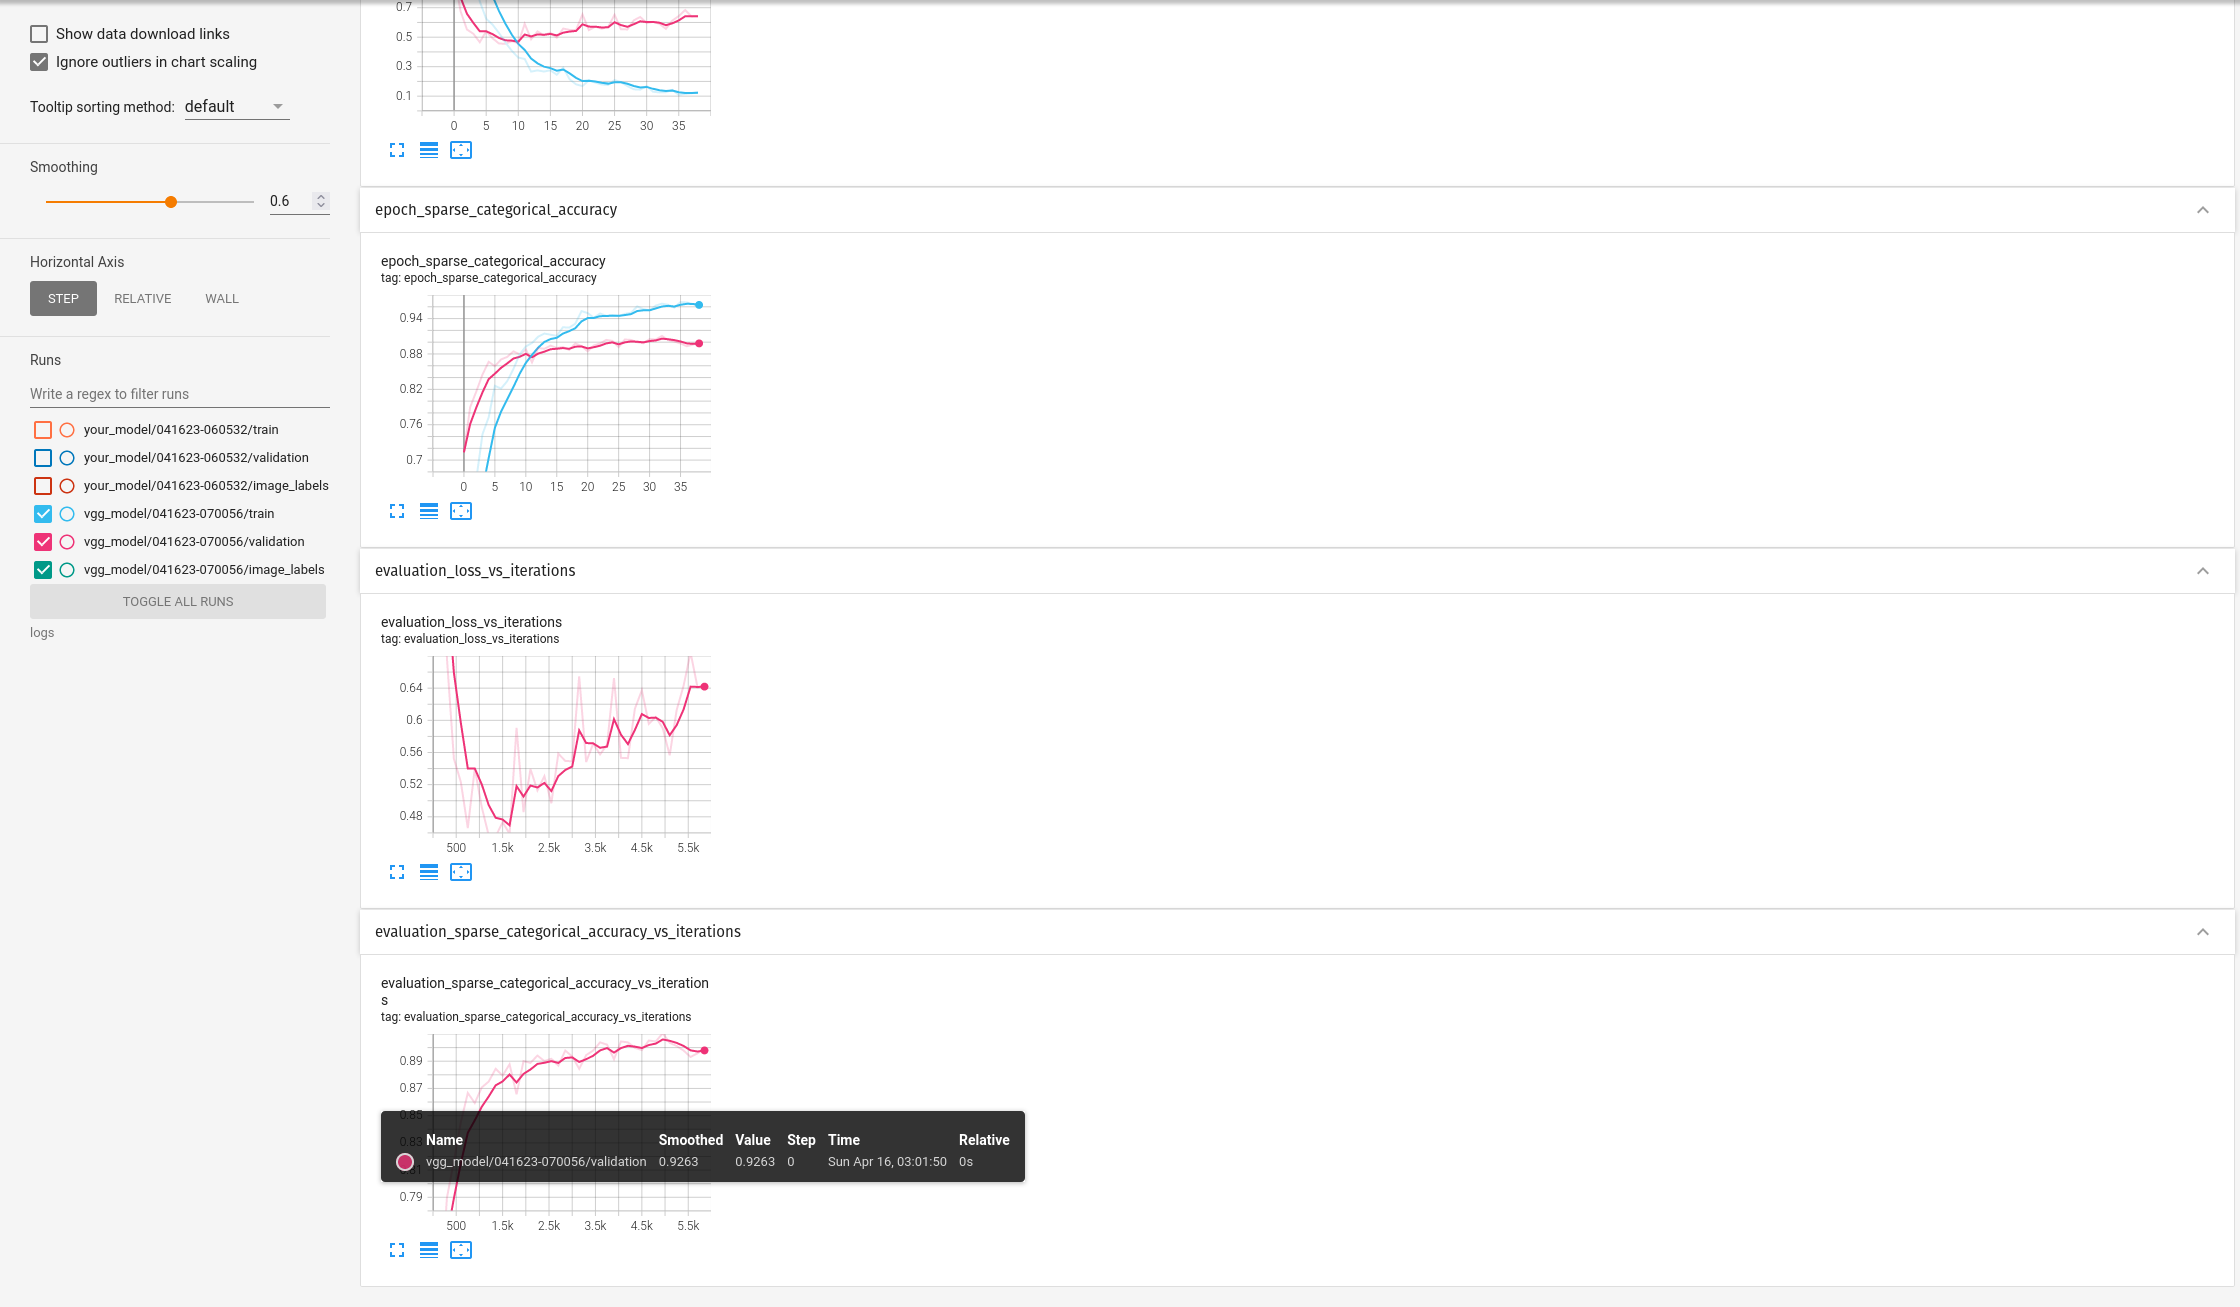
\includegraphics[width=5cm]{vgg-b.png}
    \caption{Progress training head of the vgg model.}
    \label{fig:result1}
\end{figure}

% TODO: changes to performance after adding 

\begin{table}[h]
    \centering
    \begin{tabular}{lr}
        \toprule
        With & Sparse categorization accuracy \\
        \midrule
        Base & 1 \\
        Standardization & 1000 \\
        Data augmentation & 1000 \\
        Regularization & 0.6873 \\
        \bottomrule
    \end{tabular}
    \caption{Task 1 performance after adding:}
    \label{tab:table1}
\end{table}

\begin{table}[h]
    \centering
    \begin{tabular}{lr}
        \toprule
        Type & Sparse categorization accuracy \\
        \midrule
        Total & 0.9106 \\
        \bottomrule
    \end{tabular}
    \caption{Task 3 performance}
    \label{tab:table2}
\end{table}


\begin{figure}[h]
    \centering
    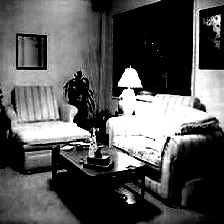
\includegraphics[width=5cm]{bedroom-should-living-room.png}
    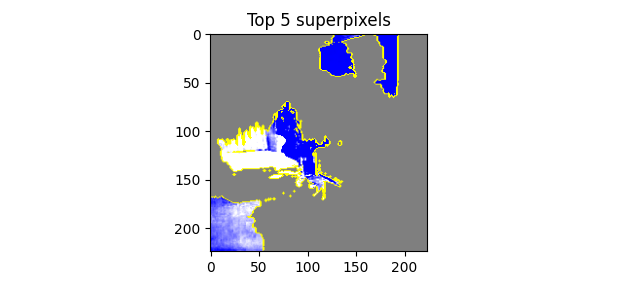
\includegraphics[width=5cm]{lime-bedroom-should-living-room.png}
    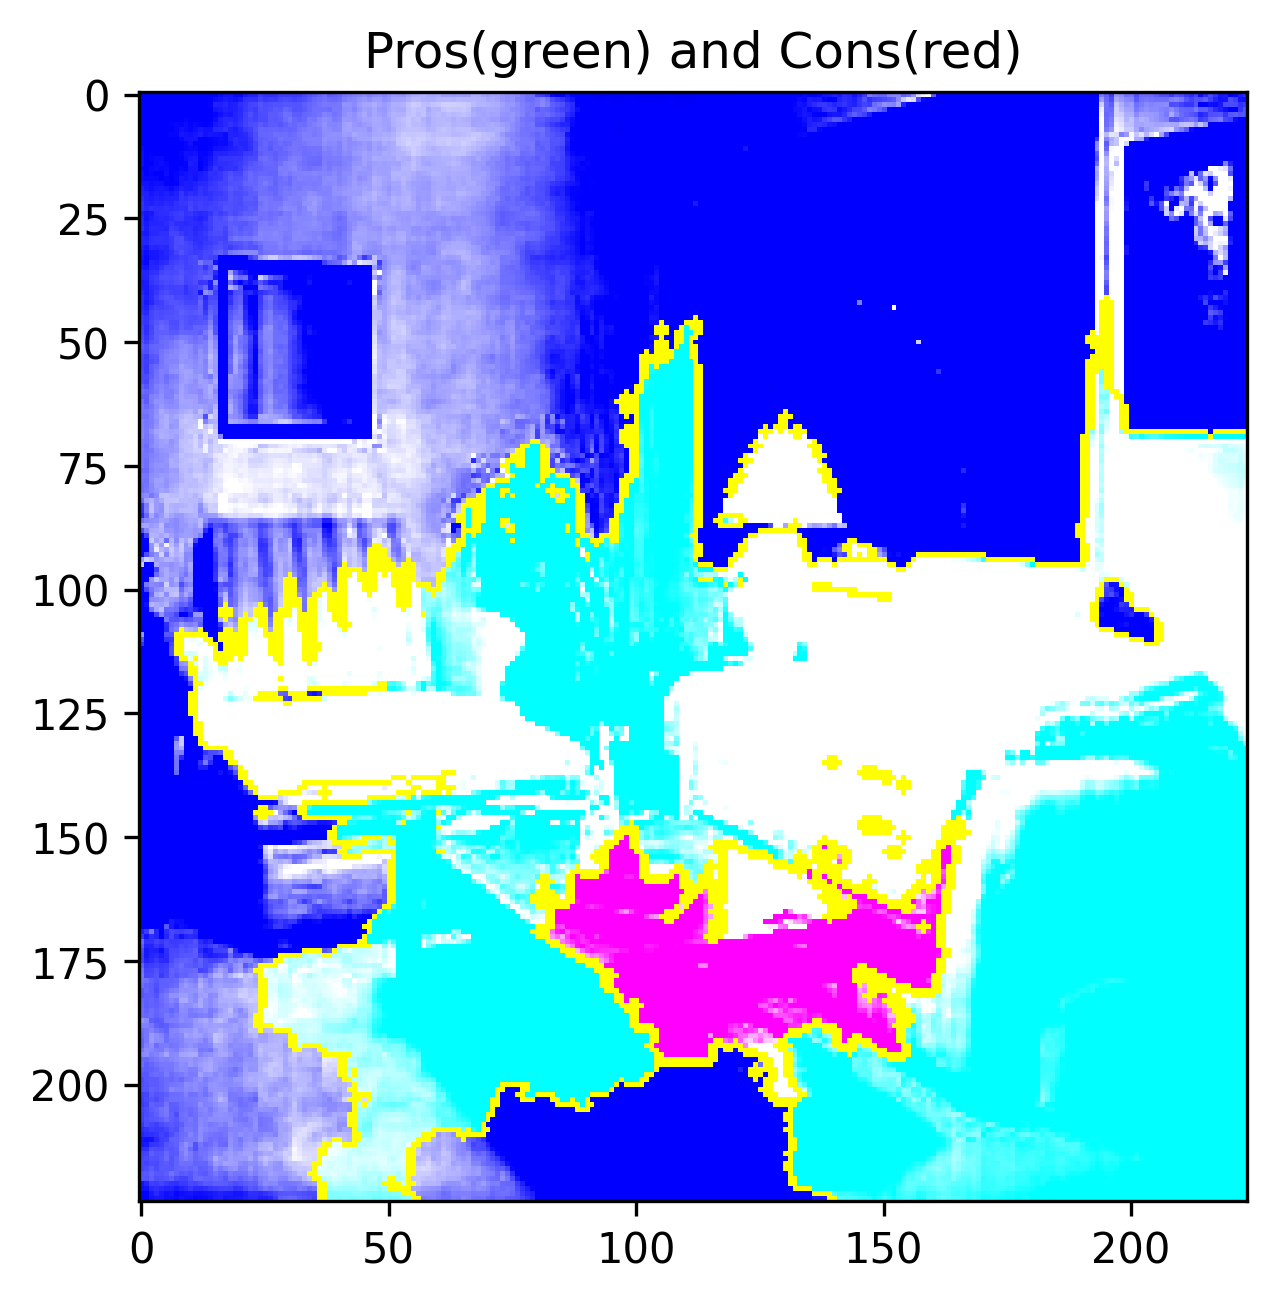
\includegraphics[width=5cm]{procon-bedroom-should-living-room.png}
    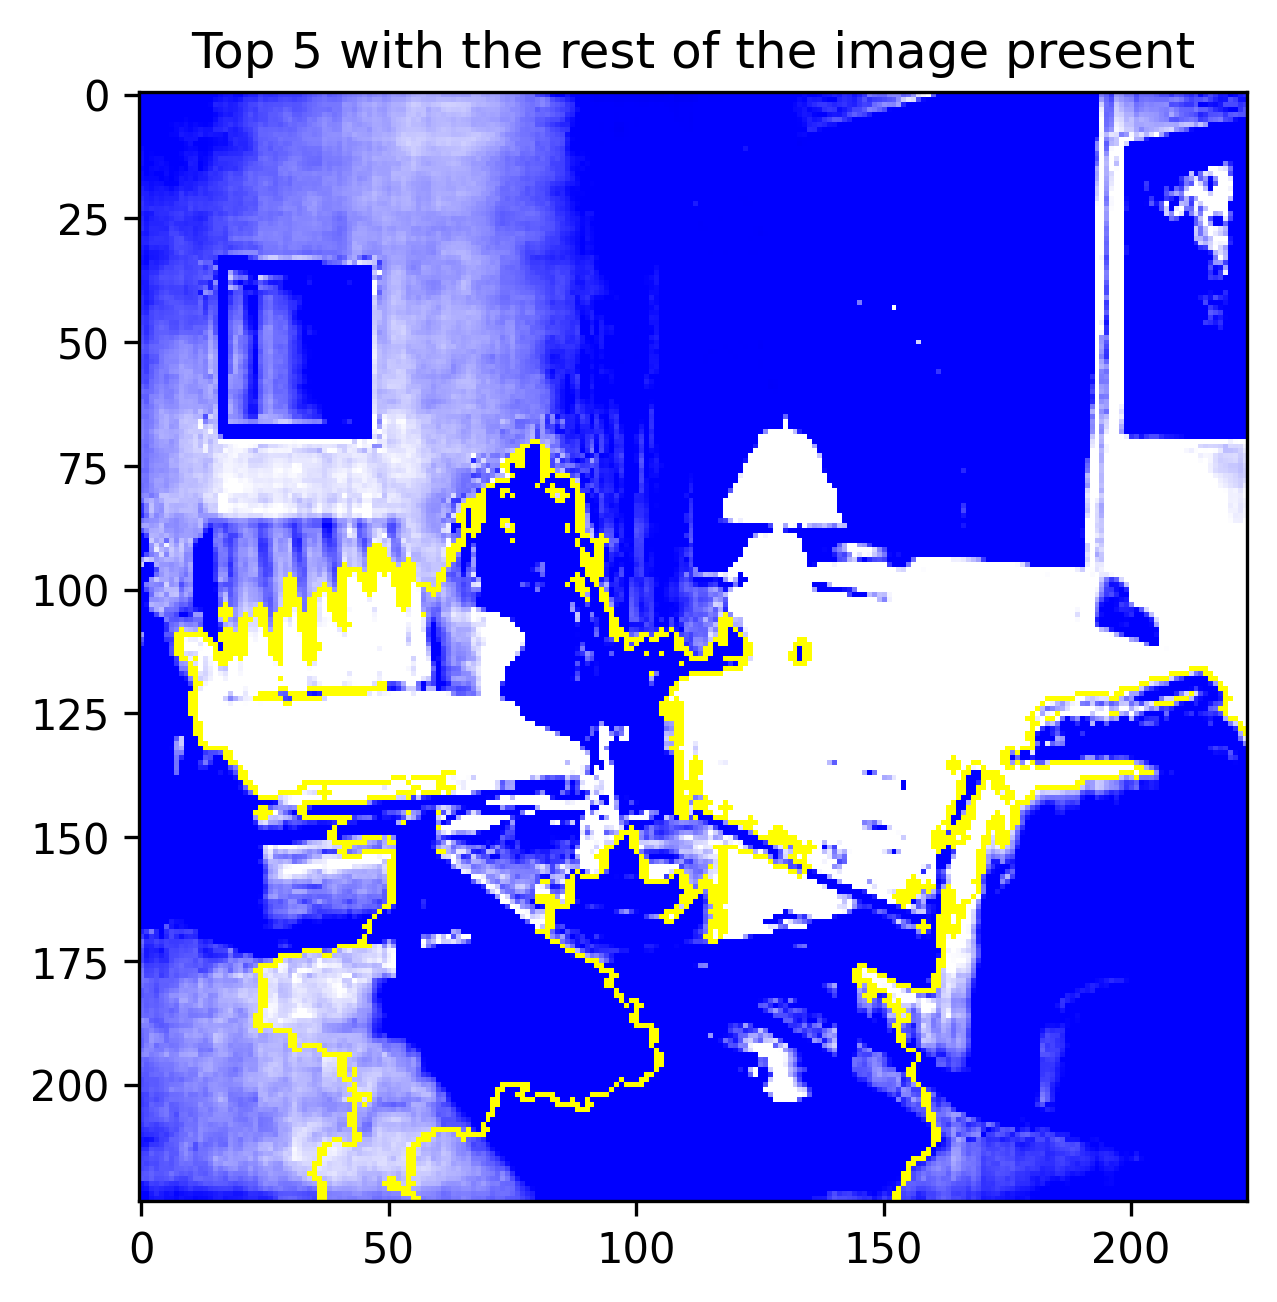
\includegraphics[width=5cm]{top5-bedroom-should-living-room.png}
    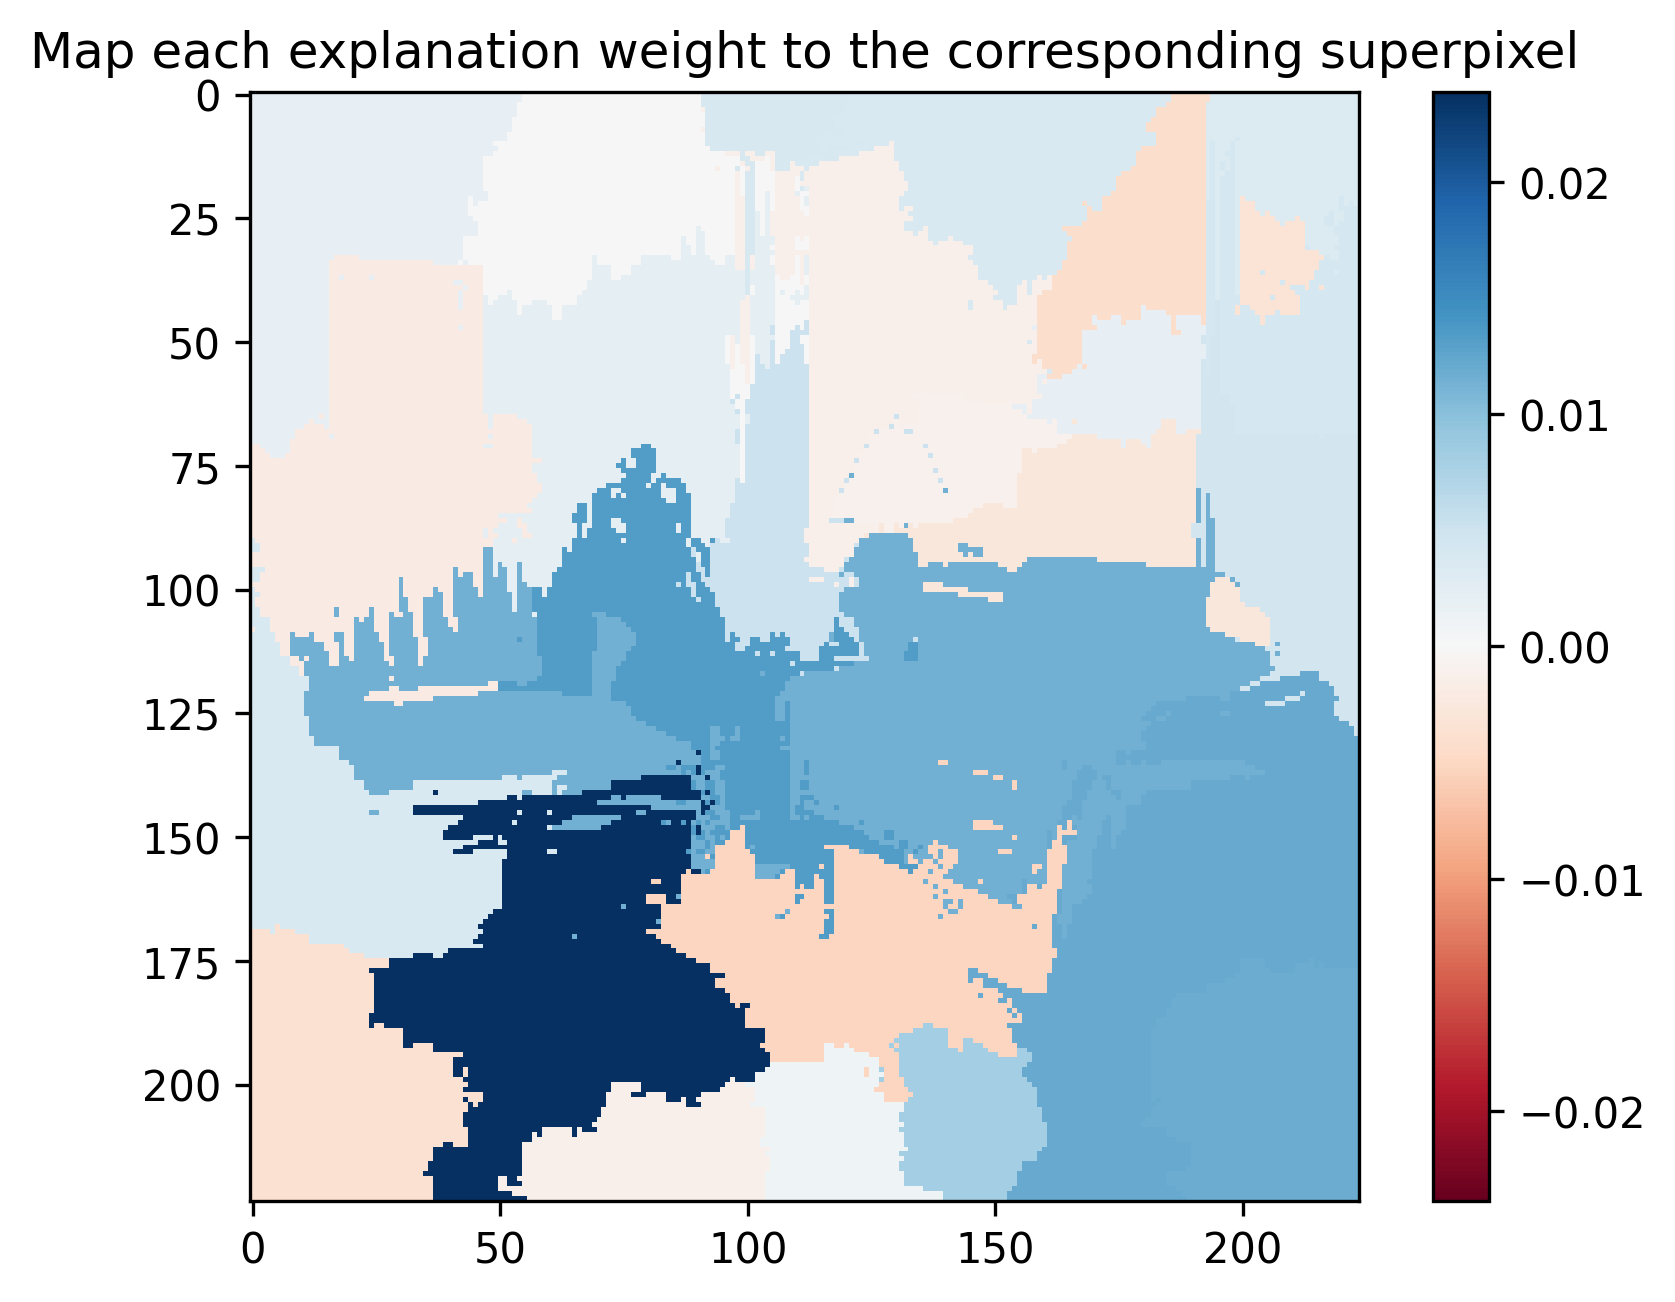
\includegraphics[width=5cm]{weight-bedroom-should-living-room.png}
    \caption{This is a bedroom, but was predicted as a living room.  Curious.}
    \label{fig:result1}
\end{figure}

\begin{figure}[h]
    \centering
    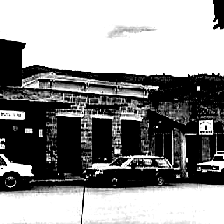
\includegraphics[width=5cm]{suburb-should-insidecity.png}
    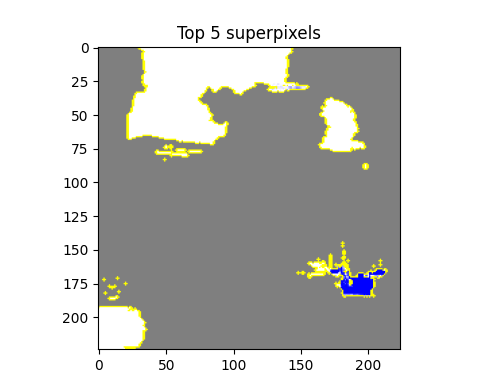
\includegraphics[width=5cm]{lime-suburb-should-insidecity.png}
    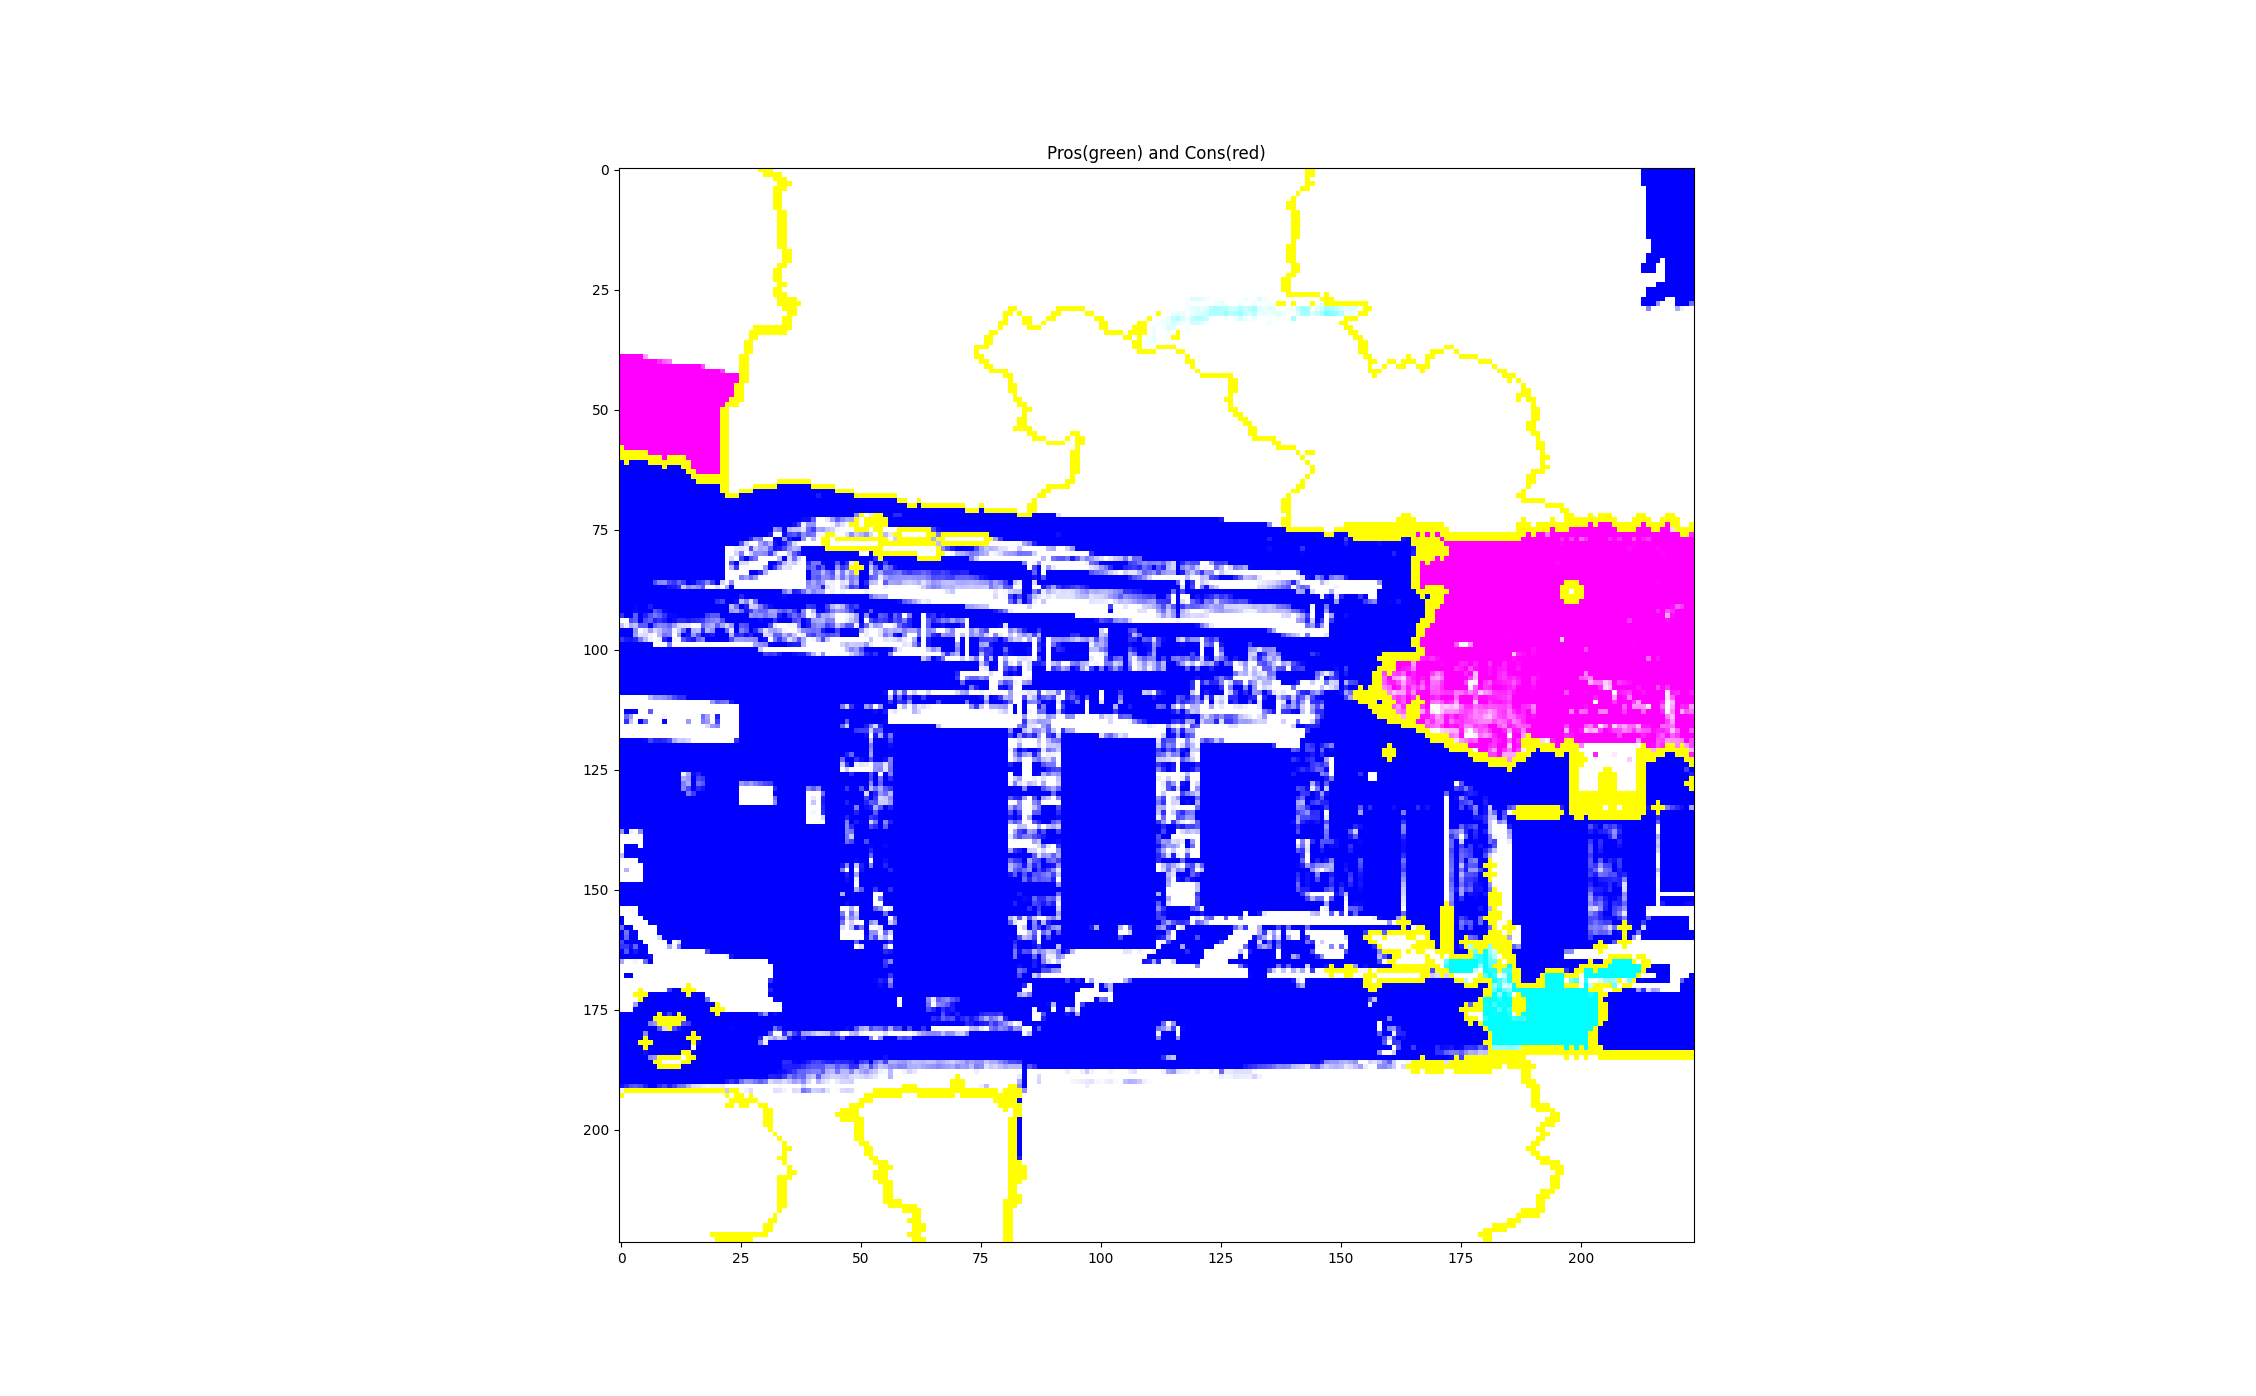
\includegraphics[width=5cm]{procon-suburb-should-insidecity.png}
    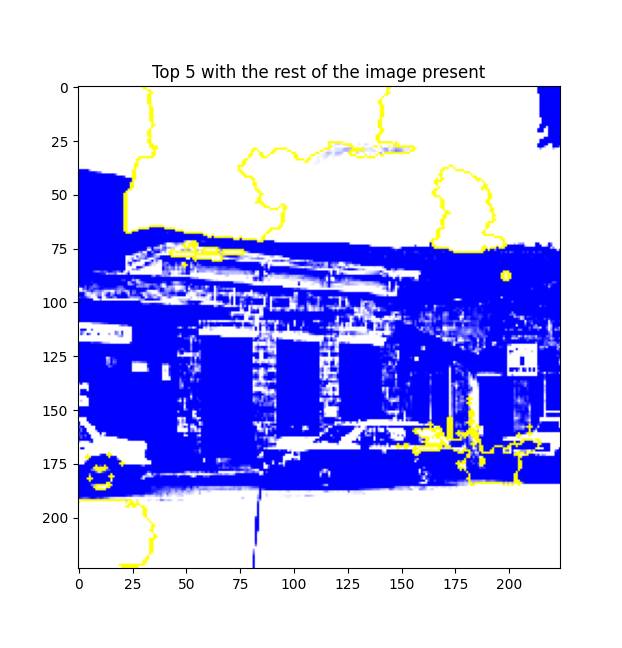
\includegraphics[width=5cm]{top5-suburb-should-inside-city.png}
    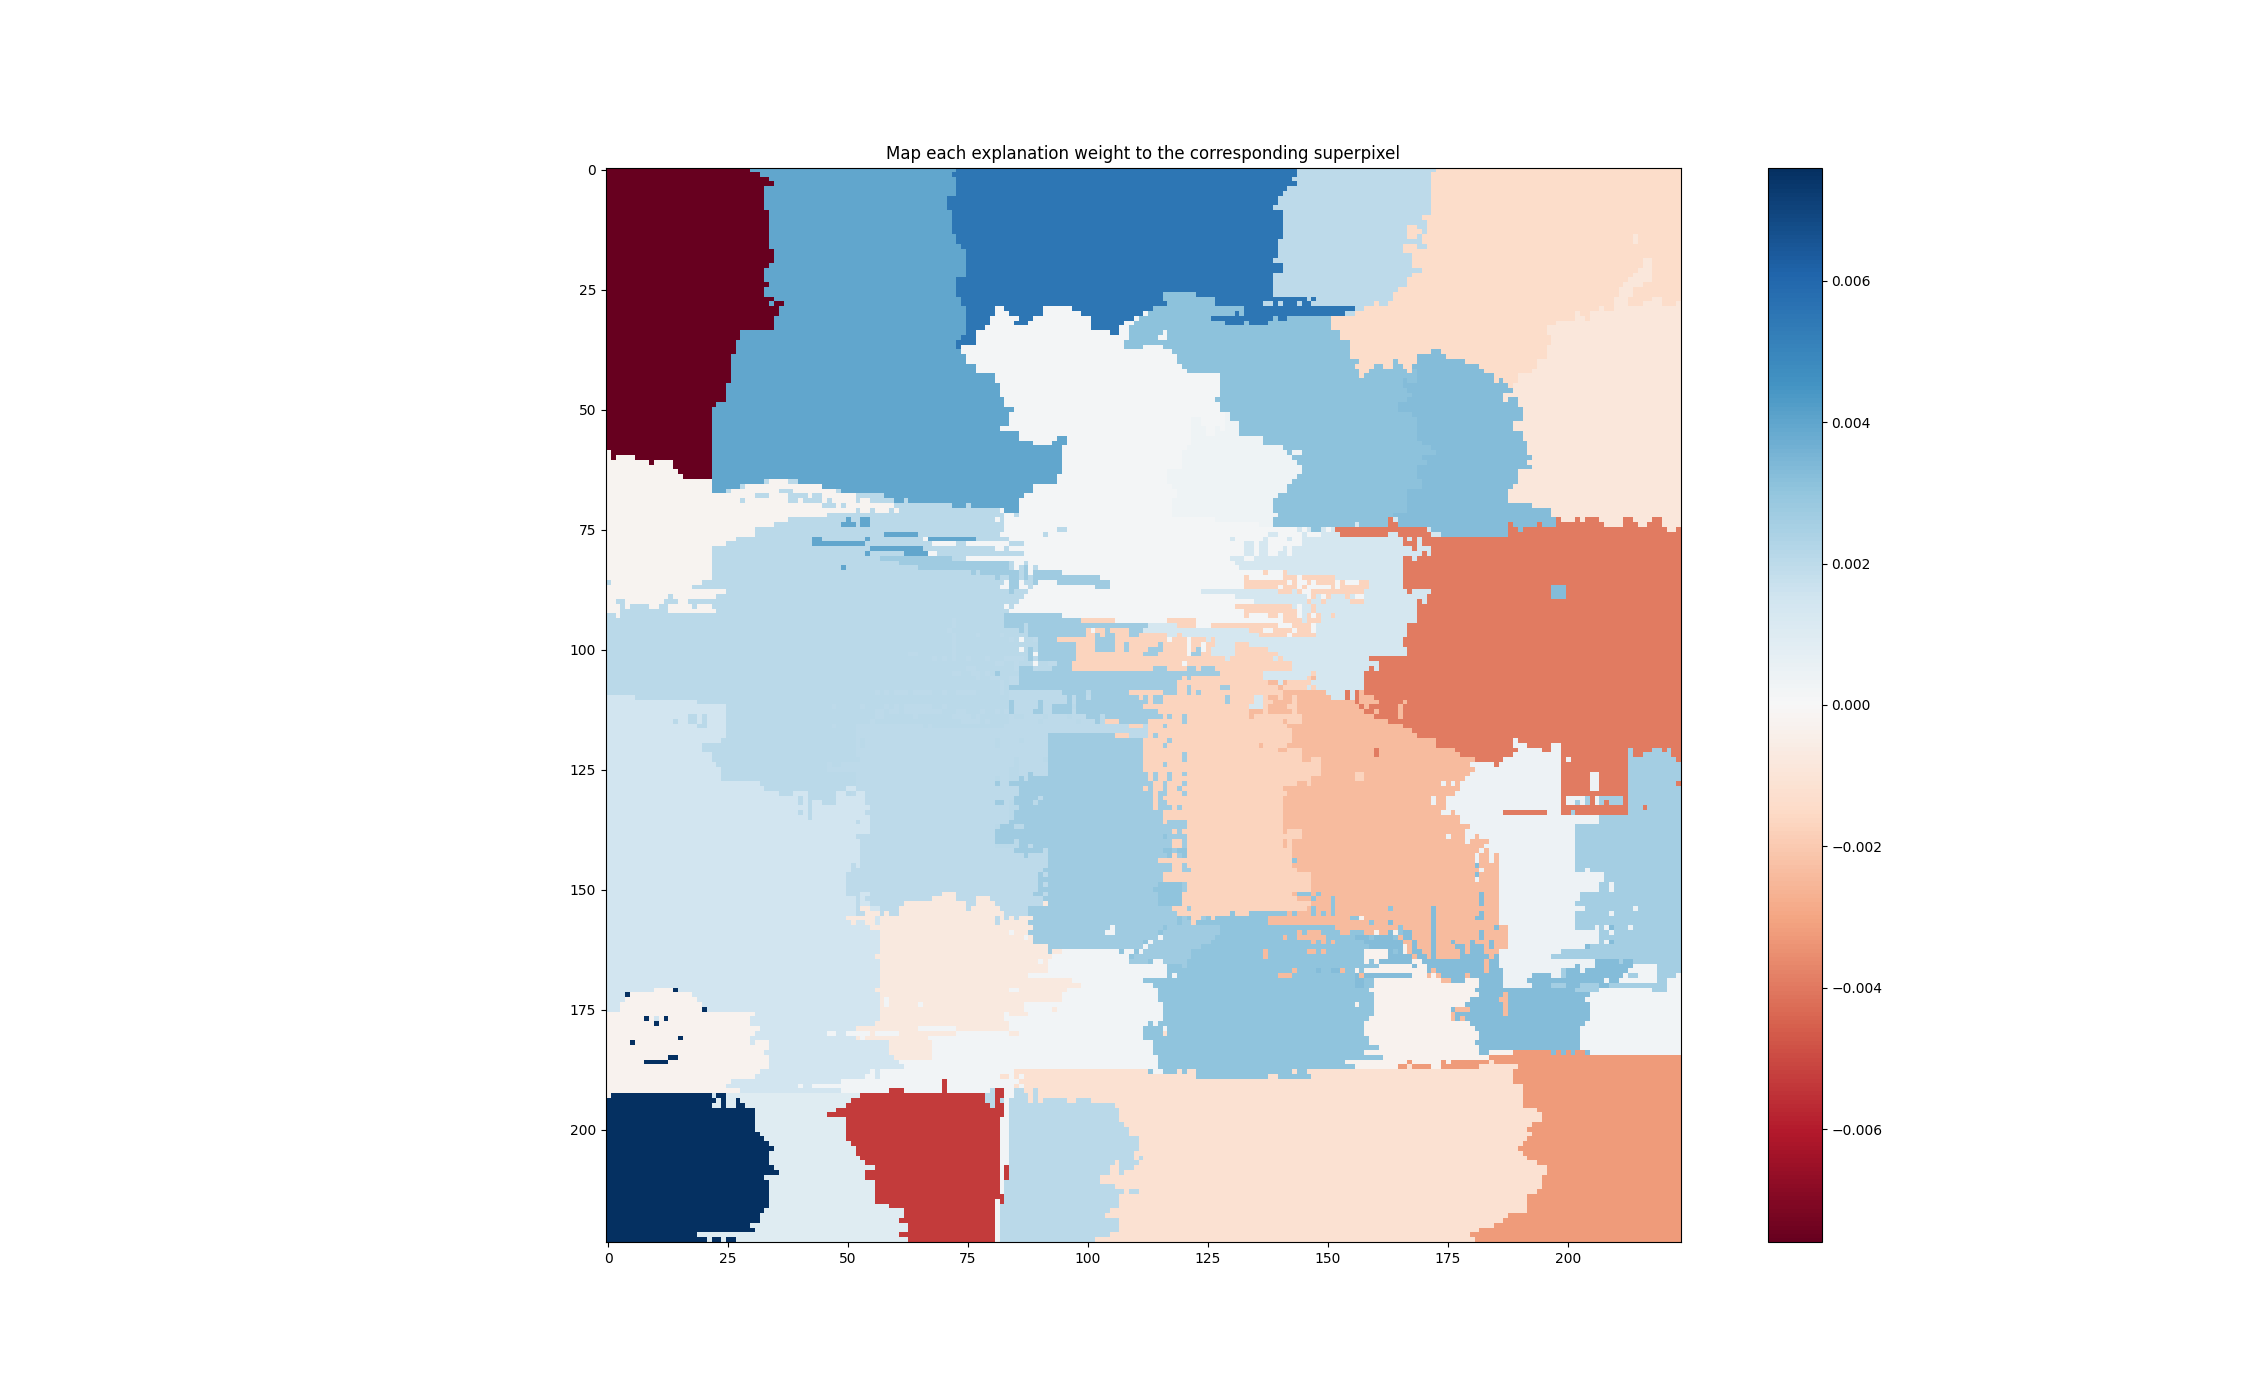
\includegraphics[width=5cm]{weight-suburb-should-insidecity.png}
    \caption{This is an inside city, but was predicted as a suburb.  Curious.}
    \label{fig:result1}
\end{figure}

% TODO: explanation

\end{document}
